
\section{Time series model}
\label{sec:model:TSMS}

Following current database models, a \acro{TSMS} model consists of two
components: a data model and a set of operations. Measures and time
series are the main objects of our \acro{TSMS} model. In both objects
time plays an important role and requires a coherent treatment.
%
We describe the \acro{TSMS} nomenclature in three
parts: the data structure model, time series manipulation and
operation, and time series specific properties.

\todo{data model inclou tot: data structure i data manipulation}

\subsection{Data model}

Roughly speaking a \emph{time series} is a set of observations
collected at specific time instants. An observation may consist of a
single attribute or multiple attributes collected at the same time
instant.  Each pair of time and observed values is refered as a
\emph{measure}. Then, a time series is a correspondence between times
and values. A time series can be described by a set of measures.

We name \emph{time domain} the set $T$ of all the possible time
values. $T$ can be either a finite or an infinite set and usually it
is a closed set. 

In this paper we will assume that the domain $T$ is the set of
affinely extended real numbers $\Rb = \R \cup
\{+\infty,-\infty\}$. Because $\Rb$ is a metric space, we can
differentiate between time instants (the elements of the set) and
durations (the metric). Next, we define the main time related concepts
using this naive approximation that avoids complex details while being
powerful enough for our purposes.

\begin{definition}(Time concepts)
  \label{def:model:temps}
  Let $T=\Rb$ be the domain for time.
  %
  We define a \emph{time instant} as an element $i$ of $\Rb$.
  %
  Let $t_i,t_j\in\Rb$ be two time instants.  We define the
  \emph{duration of time} between $t_i$ and $t_j$ as the value $t \in
  \Rb$ which measures the distance in time units between two time
  instants $t = t_i - t_j$.
\end{definition}

A value is an attribute that indicates the magnitude of a measure. The
domain for the values can be any data type. Valid domains for values
include integers, real numbers, strings, and more elaborated data
structures such as arrays, lists, or even other time series. Without
loss of generality in this paper we will assume that the domain of
values is the set of projectively extended reals $\Rp = \R \cup
\{\infty\}$.
%
\todo{Per que aqui es $\Rp$ i en el temps $\Rb$?}
%En els valors només cal extendre amb una marca d'indefinit
%Però potser per simplificar podríem fer servir Rb a tot arreu
%
Note that although we defined values as scalars it is easy to extend
the concept to multivalues which represent a collection of values
measured at the same time instant~\cite{assfalg08:thesis}.


A measure represents an actual value measured in a particular time
instant. We define it below.
\begin{definition}
  Let $v$ be a value and let $t$ be the time instant when the value
  was acquired. We define a \emph{measure} $m$ as the tuple $m=(t,v)$.
\end{definition}

Let $m = (t,v)$ be a measure. In what follows, $V(m)$ denotes the
value $v$ and $T(m)$ denotes the time $t$.

Order between mesures plays an important role. Given two measures we
define two distinct order relations.
%
\todo{Te sentit l'ordre entre mesures de fenomens diferents? L'ordre
  nomes s'ha d'aplicar a les mesures d'un mateix time series?}
%En les operacions binàries hi haurà mesures de dues sèries temporals.
%En algunes operacions es requreix que les sèries siguin del mateix tipus.

\begin{definition}[Semitemporal order]
  Let $m$ and $n$ be two measures. We name \emph{semitemporal order}
  the binary relation written $m\leq n$ and defined as $m\leq n\iff
  (T(m)<T(n) \vee m=n)$.
\end{definition}

\begin{definition}[Temporal order] Let $m$ and $n$ be two measures. We
    name \emph{temporal order} the binary relation written $m \leq^t
    n$ and defined as $m \leq^t n \iff T(m) \leq T(n)$.
\end{definition}

Note that the semitemporal order is a partial order while the temporal
order is a total order.

Intuitively speaking a time series is set of measures of the same
phenomena.  Sometimes they are also called time
sequences~\cite{last:hetland}. We define it as follows.

\begin{definition}[Time series]
  \label{def:model:timeseries}
  Let $S = \{m_0,\ldots,m_k\}$ be a set of measures of the same
  type. Then, $S$ is a \emph{time series} iff $\forall i,j:
  i,j\in[0,k] \wedge i\neq j: T(m_i)\neq T(m_j)$.
\end{definition}

Observe that although measures in $S$ are expected to be of the same
phenomena, from a formal standpoint we only require the type of all
values to be the same.
%% Per revisar aquest detall. Que vol dir que tenen un ordre total?
% En una sola sèrie temporal no hi ha mesures repetides.
% Per tant totes les mesures estan ordenades, és a dir només s'aplica l'ordre temporal. 
As there are no repeated time values, measures in a time series have a
total order.

The cardinality of a time series $S=\{m_0,\dots,m_k\}$, noted as
$|S|$, is the number of measures that contains.  A empty time series is
noted as $\emptyset$. Needless to say, $|\emptyset|=0$.

A time series can record more than one phenomena if they share the
same time instants of acquisition. Then it is a \emph{multivalued time
  series}. Let $S = \{m_0, \ldots, m_k\}$ be a multivalued time
series. We write its measures as $m=(t,v_1,v_2,\ldots,v_n)$, that is
the value has domain $(\Rp)^n$.




\subsection{Operations}
\label{sec:model:operations}

Time series have a time attribute that must be manipulated
coherently. Owing to this time attribute, the behaviour of a time
series can be handled on three ways:  set operations including
relational ones,  sequence operations, and  temporal function
operations that manipulate a time series considering it is a
representation for a continuous function. Next a brief description of
most important ones is given.


% These time series manipulations are defined abstractly for any time
% series having the structure of Definition \ref{def:model:timeseries}.
% In the same way as the relational model for operations, definitions
% evaluate algebra and logic concepts for data but do not evaluate the
% semantics of manipulations. That is, when given a particular context
% for a time series manipulation it has to be decided whether the
% algebra is meaningful or cannot be applied, for example an addition of
% values in two different units could be semantically erroneous.


\subsubsection{Set operations}

We describe how common set operators can be applied to time series. We
rely on how the relational model of \acro{DBMS} describes operations
based on set algebra~\cite{date:introduction}.


Consider a time series $S$. $S$ is a finite ordered set (by the
temporal order). Then, if $S$ nonempty, $S$ has a maximum and a
minimum.  
%
Let $S$ be a time series and $n\in S$ be a measure. The \emph{maximum}
of $S$, noted as $\max(S)$ is an element of $S$ such that $\forall m
\in S:\max(S)\geq^t m $.  
%
Note that $\max(S)$ is not defined when $S=\emptyset$. However, the
time series has a supremum even when empty. In fact, according to~
\cite{cantrell:extendedreal}, $\sup(\emptyset)=-\infty$.
%
Using this fact we define the \emph{supremum} os $S$, noted as
$\sup(S)$, as $\sup(S)=\max(S)$ when $S$ non empty or
$\sup(S)=-\infty$ otherwise.
%
Dually, we can define the \emph{minimum} of $S$, noted as $\min(S)$,
and the \emph{infimum} of $S$, noted as $\inf(S)$.

%%%%%%%%% Paragra per repassar en segona volta
In time series binary set operations, the measures can have the two
possible order relations: temporal and semitemporal. Consequently,
these two possible order relations of measures impose two operation
definitions for some set operators.  Mainly they impose two membership
operations and so to all operations based on it.
%%%%%%%%%

The membership operation defines when a measure belongs to a time
series. We define two distinct membership operations. This induces two
different ways to consider time series and its operations.


Let $S$ be a time series and $m$ be a measure. 
%
We say that $m$ belongs to $S$ (plain \emph{membership}), denoted as
$m \in S$, when $\exists x\in S: x=m$.  We also say that $m$ belongs
temporally to $S$ (\emph{temporal membership}), noted $m \inst S$,
when $\exists x\in S : T(m)=T(x)$.


The two distinct membership criteria induce two meanings for
inclusion. Let $R$ and $S$ be two time series.  We say that $R$ is
\emph{included} in $S$, written $R\subseteq S$, when all the elements
of $R$ belong to $S$.  Analogously, we say that $R$ is \emph{included
  temporally} in $S$, noted $R\subseteqt S$, when all the elements of
$R$ belong temporally to $S$.


The \emph{union} of two sets is a set containing elements from both
sets. Usual set union operations do not apply to time series because
the result time series could have repeated time values.  Then, we will
give a slighty modified concept for union.
% PER ARRANJAR
Again, two versions of the union will appear according to the 
XXXX
%

The union requires both time series to have the same structure and
type as happens with union operation in relational \acro{DBMS}
\cite{date:introduction}.\todo{I la resta d'operacions no?. Aquest
  concepte s'escapa una mica per que es semantic. En un moment de
  l'article es dir que s'assumeix que els valors son sempre reals.}
%Sí, la diferència i intersecció tambés es requereix. 
%Cal pensat en mateixa estructura alhora en el sentit de tipus i de sèrie temporal multivaluada

%
Let $R$ and $S$ be two time series. 
%
The \emph{union} of $R$ and $S$, noted $R\cup S$, is a new time series
$R \cup S = \{m|m\in R\vee (m\in S\wedge m \notinst R)\}$. 
%
The \emph{temporal union} of $R$ and $S$, noted $S_1 \cupt S_2$, is a
time series $R \cupt S = \{ m | (m \in R \wedge m \in S) \vee (m \in R
\wedge m \notinst S) \vee (m \in S \wedge m \notinst R) \}$.  \todo{te
  sentit en la unio el concepte 'temporal'? te el mateix sentit que a
  la pertanyensa? No aplicaria millor el concepte 'unio simetrica'?}
%
It is interesting to emphasize that union is a non commutative
operation while temproal union is a commutative one.

\begin{figure}
  \centering
  %\def\escala{0.9}

\def\nodeA{node [above left=0.5cm and 0.1cm] {$(1,1)$} node [below left=0.5cm and 0.1cm] {$(5,1)$}}
\def\nodeB{node [above right=0.5cm and 0.1cm] {$(2,2)$} node [below right=0.5cm and 0.1cm] {$(6,2)$}}
\def\nodeT{node [above=0.1cm] {$(4,0)$} node [left=0.4cm] {$(3,1)$} node [right=0.4cm] {$(3,2)$}}
% Definition of circles
\def\firstcircle{(0,0) circle (1.5cm)}
\def\secondcircle{(0:2cm) circle (1.5cm)}
\def\thirdcircle{(0:1cm) circle (1.11cm)}

\colorlet{circle edge}{blue!50}
\colorlet{circle area}{blue!20}

\tikzset{
  filled/.style={fill=circle area, draw=circle edge, thick},
  outline/.style={draw=circle edge, thick},
  every node/.style={transform shape}
}

%\setlength{\parskip}{5mm}






%Set A or B
\begin{tikzpicture}[scale=\escala]
  \draw[filled] \firstcircle \nodeA;
    \begin{scope}
        \clip \secondcircle;
        \draw[filled, even odd rule] \firstcircle \nodeA
                                 \secondcircle 
                                 \thirdcircle;
   \end{scope}
    \draw[outline] \firstcircle
                   \secondcircle \nodeB
                   \thirdcircle \nodeT;

   \node[anchor=south] at (current bounding box.north) {$S_1 \cup S_2$};
\end{tikzpicture}
%Set temporal A or B
\begin{tikzpicture}[scale=\escala]
    \draw[filled, even odd rule] \firstcircle \nodeA
                                 \secondcircle \nodeB
                                 \thirdcircle \nodeT;
    \node[anchor=south] at (current bounding box.north) {$S_1 \cup^t S_2$};
\end{tikzpicture}






%%% Local Variables:
%%% TeX-master: "../main"
%%% ispell-local-dictionary: "british"
%%% End:

  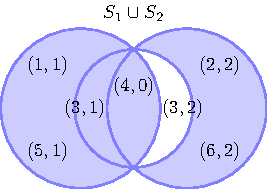
\includegraphics{fig_model_venn.pdf}
  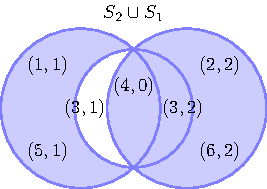
\includegraphics{fig_model_venn_reverse.pdf}
  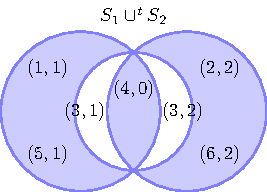
\includegraphics{fig_model_venn2.pdf}
  \caption{Venn diagrams for set and temporal set union operations of
    \acro{TSMS}}
  \label{fig:model:venn}
\end{figure}


\begin{example}\label{ex:model:s1s2}
  Let $R=\{(1,1), (3,1), (4,0), (5,1)\}$ and $R=\{(2,2), (3,2), (4,0),
  (6,2)\}$ be two time series. The union of $R$ and $S$ is $R\cup
  S=\{(1,1), (2,2), (3,1), (4,0), (5,1), (6,2)\}$. Because union is
  not symmetric, $R\cup S=\{(1,1), (2,2), \allowbreak(3,2), (4, 0), (5,1),
  (6,2)\}$. The temporal union results in $R\cupt S= S \cupt
  R=\{(1,1), (2,2), (4,0), (5,1), (6,2)\}$.  
  %
  Venn diagrams for all three cases are shown in
  Figure~\ref{fig:model:venn}, where the coloured area depicts the
  result time series. In every diagram, the central intersection area
  contains measures that share both time and value attributes, like
  instance $(4,0)$. The central left area contains the measures in $R$
  that only share the time attribute with a measure in $S$, like
  instance $(3,1)$. The central right area has a symmetrical
  meaning. The left and right outer areas are the remaining measures
  of $R$ and $S$ respectively.
\end{example}




Time series \emph{difference} can also be defined. Like union, the
difference requires both time series to have the same structure.
%
Let $R$ and $S$ be two time series.
%
The \emph{difference} between $R$ and $S$, written $R-S$, is a time
series $R-S=\{m|m\in R\wedge m\notin S\}$.
%
The \emph{temporal difference} between $R$ and $S$, denoted $R-^t S$, 
is a time series $R-^tS=\{m|m\in R\wedge m \notinst S\}$.


Based on union and difference we can define \emph{intersection} as
$S_1\cap S_2 \equiv S_1 - (S_1 - S_2)$ and \emph{symmetric difference}
as $S_1 \ominus S_2 \equiv (S_1 - S_2) \cup (S_2 - S_1)$. The
corresponding temporal operations can also be defined.


Relational \acro{DBMS} extend set operators with specific ones like
projection, selection, rename, product or join. This kind of operators
also make sense for time series. To illustrate this possibility we
define the join operator.

Roughly speaking, the join of two time series is the grouping of
measures sharing the same time attribute.  Let $R$ and $S$ be two time
series.  The \emph{join} of $R$ and $S$, denoted $R \join S$, is a
multivalued time series $R \join S = \{ (t,v_1,v_2) | (t_1,v_1) \in
R\wedge (t_2,v_2) \in S \wedge t=t_1=t_2 \}$.  \todo{Potser allo que
  es diu al principi que nomes es consideren series univaluades s'ha
  de repassar}


A \acro{DBMS} requires computational operators to provide opportunity
to calculate using the data contained. Relational \acro{DBMS} supply
operators like extend, aggregate or
summarise~\cite{date:introduction}. For time series, we define the more
general computational operators map and fold.
\todo{Aqui s'escauria una citacio indicant l'origen d'aquests operadors}
%Són molt genèrics, no sé d'on podríem treure una referència

The map operator transforms a time series by applying a function to
every measure.  Let $S$ be a time series and let $f:m\mapsto m'$ be a
function over a measure returning a measure. The \emph{map} of $f$
over $S$ is a new time series defined as $\map(S,f)=\{f(m)|m\in S\}$.

The fold operator recursively combines every measure of a time series.
%
Let $S=\{m_0,\dots, m_k\}$ and $R$ be two time series and let $f:
S\times m \mapsto S'$ be a function over a time series and a measure
returning a time series. 
%
The \emph{fold} of $S$ by $f$ with initial value $R$ is a new time
series defined as $\fold(S,R,f) = f(\cdots(f(f(f(R,m_0),\allowbreak
m_1),\allowbreak m_2)\cdots),\allowbreak m_k)$.

The classical aggregation operator is used to combine the data of a
time series into a single value.  It is worth to note that it is a
specific case of fold.
\todo{S'hauria d'explicitar per que es un cas particular}
%Doncs potser eliminar aquesta frase? 
%Prové que abans ho definíem a partir dels fold però ara, per simplificar, ja no.

Let $S=\{m_0,\dots,m_k\}$ be a time series, let $m$ be a measure and
let $f$ be a function over two measures returning a measure. The
\emph{aggregate} of $S$ by $f$ with initial value $m$ is a new time
series defined as $\agg(S,m,f) = f(\cdots(f(f(f(m,m_0),\allowbreak
m_1),\allowbreak m_2)\cdots),\allowbreak m_k)$.  \todo{hi ha un
  problema notacional en definir les funcions per que no esta definit
  el conjunt universal de mesures. Potser millor definir-ho de paraula
  com en aquest darrer paragraf.}

%A more generic version of fold is a fold considering order. 
In the previous fold, the measures are computed in random order.
However in some computational operations it is necessary to define the
order, especially when $\ffold$ is not commutative.
\todo{No te sentit parlar de commutativitat d'una funcio}
Then, it is possible
to define a \emph{fold with order} as an extension of fold where
measures are computed in a predetermined order.

% We define a
% \emph{fold with order}, $\orderfold$, as an extension of fold with a
% function $o$ that selects measures in order where $o: S_a \mapsto m_r$
% \[
%  \orderfold(S,S_i,f^f,o) =
%   \begin{cases}
%     S_i  \text{ if } |S|=0, \\
%     \orderfold(S_o,f^f(S_i,m_o),f^f,o)  \text{ else}
%   \end{cases}
% \]
% where $m_o = o(S)$ and $S_o = S - \{m_o\}$.



\begin{example}
\label{ex:computational-operators}
Let $S=\{(1,1),(2,3),(4,1)\}$ be a time series.  Map operator allows
computing a new time series whose values result from time multiplied
by value.  We define the map function $f(t,v)=(t,t\cdot v)$. Then
$\map(S,f)=\{(1,1),(2,6),(4,4)\}$.  \todo{times es pel producte
  cartesia}

The aggregate operator allows, for instance, to compute the measure
that results from the sum of all the values.  To illustrate it, we
define the aggregate function $f(m,n)=(0,V(m)+V(n))$. Now,
$\agg(S,(0,0),f) = (0,5)$, the sum of all the values of $S$. Note that
time is meaningless in this computation.

The fold operator allows, for instance, to select the measures having
its value equal to one.  We define the fold function $f(S,m)=S\cup S'$
where $S'=\{m\}$ if $V(m)=1$ or $S'=\emptyset$ otherwise. Then
$\fold(S,\emptyset,f)=\{(1,1),(4,1)\}$.
\end{example}

%%%%%%% BINARY COMPUTATIONAL OPERATORS

Finally we describe how, using the operators defined before, we can
implement \emph{binary computational} operators between two time
series. This illustrates the power of the operators defined so far.
%

The strategy requires first to join the two time series and then
apply the computational operations. 
%
Let $S$ and $R$ be two time series and $\odot$ be a binary operator on
the value domain. The operator $\odot$ can be extended to the time
series as:
%
$S\odot R=\map(S\join R, f)$ being $f$ the funcion
$f(t,v,w)=(t,v\odot w))$.
%
This allows to extend real binary operations such as sum or division
to time series.  \todo{Epsss aixo del join cal explicar-ho quan es
  parla del join!!!! es important}
%Sí, totalment!
It must be noted that join requires both time series
to have exactly the same time attribute. When time series diverge too
much then temporal function operations can be applied to fit the time
instants to what is required.





\subsubsection{Sequence operations}

Sequence operations manipulate time series considering measures as
being totally ordered. Then three basic operations can be defined:
interval, successor and concatenation.


The \emph{interval} $(t_i,t_j)$, where $t_i$ and $t_j$ are two time
instants, over a time series $S$ is a time subseries between the two
time instants $S(t_i,t_j) \subseteq S$. A similar interval concept
is used by \cite{last:hetland}. The open interval is defined as
$S(t_i,t_j)=\{m | (m\in S) \wedge (t_i<T(m)<t_j)\}$. Other intervals can be
defined: closed $S[t_i,t_j]$, left-open $S(t_i,t_j]$, and right-open
$S[t_i,t_j)$.

The time order in time series also implies the sequence concept of
\emph{successor} and \emph{predecessor}.  Let $S=\{m_0, \ldots, m_k\}$
be a time series, $m_i\in S$ a measure and $m$ another measure. We
say $m_i=\nex_S(m)$ is the \emph{next} measure to $m$ in $S$ if
and only if $m_i=\inf(S(T(m),+\infty])$.  We say $m_i=\prev_S(m)$
is the \emph{previous} measure to $m$ in $S$ if and only if
$m_i=\sup(S[-\infty,T(m)))$. %
Infinite measures are obtained when next and previous are applied to
supremum and infimum measure respectively: $\nex_S(\sup
S)=(+\infty,\infty)$ and $\prev_S(\inf S)=(-\infty,\infty)$.



\emph{Concatenation} comprises the measures of the first time series
followed in time order by the measures of the second. It is similar to
union for sets but considering the sequence interval. The
concatenation requires both time series to have the same structure as
seen with union operation.  Let $S_1$ and $S_2$ be two time series.
 The concatenation of both $S_1 || S_2$ is a time series $S$ containing
all measures of $S_1$ and those of $S_2$ that not intersect in the
time interval of $S_1$.  $S_1 || S_2 = S_1 \cup ( S_2 - S_2[t_i,t_j]
)$ where $t_i=T(\inf S_1)$ and $t_j=T(\sup S_1)$.



\subsubsection{Temporal function operations}
\label{sec:model:tfunc}

A time series is a discrete representation of a continuous function,
more precisely a temporal continuous function as time is the function
domain. Operations that manipulate time series according to this
temporal function nature can be defined.

The \emph{graph of a function} allows to obtain and interpret the
continuous nature of a time series, when the domain of time and value
attributes can be plotted then the graph is equivalent to a graphical
representation.  Let $S$ be a time series and $T$ the time domain. The
\emph{graph} of the time series is a set of ordered pairs $\graph S =
\{ (t,S(t)) | t\in T \}$ where $S(t)$ is a temporal representation
function for the time series.

The \emph{temporal representation function} $S(t)$ is a continuous
function along variable $t$ in the domain of time and the target in
the domain of values. $S(t)$ can be obtained by various methods, so
there are several possible temporal representation functions. In all
temporal function operations a superscript $r$ indicates the name $r$
of the representation method used, as instance $S(t)^r$ is the
representation function using method $r$. We exemplify the
representation functions using two methods $r$ based on impulse and
constant piecewise functions.


\begin{definition}
  \emph{Dirac delta} (\dd) is a method of representation based on the
  Dirac delta function. It is an impulse train function that is zero
  everywhere except at zero.  Let $S$ be a time series. We define
  $S(t)^\dd$ as the \emph{\dd{} representation function}
\[
    \forall m \in S: S(t)^\dd
    =  \begin{cases}
      V(m) & \text{if }  t=T(m) \\
      0 & \text{otherwise}
    \end{cases}
\]
\end{definition}

\begin{definition}
  \emph{Zero-order hold everted} (\zohe{}) is a method of
  representation based on the \emph{zero-order hold} signal
  reconstruction methods. It is a piecewise constant function that has
  left-continuous step functions.  Let $S$ be a time series. We define
  $S(t)^\zohe$ as the \emph{\zohe{} representation function}, $\forall
  m \in S:$
\[
    S(t)^\zohe 
    = \begin{cases}
      0 & \text{if }  t > T(\max(S)) \\
      V(m) & \text{if } t\in \big(T(\prev_S(m)),T(m)\big]
    \end{cases}
\]
\end{definition}




The concept of representation is used for formalising some set and
sequence operators as temporal operators. 

%Consequently, the result of each one will depend on a representation method, which is indicated as a parameter.


We define a temporal interval operation to introduce this concept.
Let $S$ be a time series, $[t_i,t_j]$ a interval of two time instants
and $r$ a representation function. The \emph{temporal interval} noted
as $S[t_i,t_j]^r$ is a time series with measures in the interval
temporal range, $S[t_i,t_j]^r\equiv S(t)^r$ for all $t \in [t_i,t_j]$. This
is a general definition difficult to implement, so for every
representation a particular temporal interval must be interpreted:

\begin{itemize}
\item Let $S(t)^\dd$ be the \dd{} representation for $S$. The
  \emph{\dd{} temporal interval} is $S[t_i,t_j]^\dd = S[t_i,t_j]
  \cup \{m_i\} \cup \{m_j\}$ where $m_i=(t_i,0)$ and $m_j=(t_j,0)$.

\item Let $S(t)^\zohe{}$ be the \zohe{} representation for $S$. The
  \emph{\zohe{} temporal interval} is $S[t_i,t_j]^\zohe{} = S(t_i,t_j]
  \cup \{m_j\}$ where $m_j=(t_j,v)$ and $v= V(\inf( S[t_j,+\infty] ))$.
\end{itemize}



From temporal interval other operators can be defined such as temporal
selection, temporal concatenation, or temporal join. As example the
definition of temporal interval operation is given.


The temporal selection over a time series allows to change the
resolution in the context of a representation function.  Let $S$ be a
time series, $T=\{t_0,t_1,\dotsc,t_n\}$ a set of time instants, and
$r$ a representation function. The \emph{temporal selection} noted as
$S[T]^r$ is a time series with measures in $T$ times computed in
coherence with the representation function $r$: $S[T]^r = S[t_0,t_0]^r
\cup S[t_1,t_1]^r \cup \dotsb \cup S[t_n,t_n]^r$. Let $t_i$ be a time
instant, note that temporal selection depends on the temporal interval
operation $S[t_i,t_i]^r$, which is equivalent to the notion of
temporal representation function over an argument as $S[t_i,t_i]^r
\equiv \{ (t_i, S(t_i)^r) \}$.





\subsection{Properties}
\label{sec:model:properties} 

In the acquisition of data it is difficult to obtain ideal times
series as described. Following we note some properties of time series
that can be problematic when manipulating them.

First, clock is a crucial measuring instrument in time
series. Precision and accuracy is very important in timestamps.  In
\cite{kopetz11:realtime} these concepts are well described as well as
solving methods, especially clock synchronisation methods.


Second, unknown data can corrupt the database. Unknown data appear
when data have not been captured or when they have been acquired
erroneously. Then data validation must be performed, which can result
in rejecting new values if they are not correct or in reconstructing
these erroneous data.  Data validation process has to consider when
values are outside the possible range domain, when there has not been
possible to acquire a sample, when the time of acquisition between
measures is not considered freshness, etc. \acro{MTSMS} is designed to
cope with this data validation process with the help of time series
representation functions such as \zohe{}.


Third, enormous quantity of data difficults computations.  Time series
come from data recollected at monitoring systems and so their size gets
very big as continuously new measures are added.  \acro{MTSMS} is
designed to be an storage solution with data size reduction by using
time series aggregate operations.


Forth, sample period irregularities difficult later time series
analysis. That is when data have not been acquired uniformly at time it
is harder to apply join operations between time series and it do not
allow to apply time series analysis algorithms defined for sequences
approaches.  \acro{MTSMS} tries to storage regular time series in the
process of consolidation.  Next we detail the regular concept for time
series.


A time series is regular when its measures are equi-spaced in time,
according to \cite{last:hetland}. Let $S$ be a time series, $i$
be a time instant and $d$ be a time duration. Then the time
series' measures can be located in the time interval $I_0=[i,
i+d]$ and its multiples $I_n=[i+nd, i+(n+1)d]$
for $n=0,1,2,\ldots$. When time series' measures are equally spaced we
say it to be regular.

\begin{definition}
  Let $S=\{m_0,$ $\ldots,$ $m_k\}$ be a time series and $d$ a time
  duration. $S$ is \emph{regular} if and only if $\forall m \in
  S(T(\min(S),+\infty):T(m) - T(\prev_S(m)) = d$.
\end{definition}


If a time series is not regular, it can be regularised by the temporal
selection operation. Let $S$ be a time series, $i$ and $d$ the
desired regularity parameters, and $k\in\N$ a limit for the scope of
the range.  A regularised $S$ is obtained with $S[T]^r$ where $T =
\{i+nd | n\in\N \wedge n\leq k \}$ is a set of time instants equi-spaced.





\section{Multiresolution model}
\label{sec:MTSMS}


The \acro{MTSMS} are \acro{TSMS} that store time series with a lossy
compression approach, that is some data are selected and spread
in different time resolutions. The \acro{MTSMS} model is based on the
concepts of measures and time series as defined in
Section~\ref{sec:model:TSMS} and we call multiresolution time series
to each time series stored in a multiresolution database
(\acro{MTSDB}).


The architecture of \acro{MTSMS} model for one multiresolution time series is
shown in Figure~\ref{fig:model:mtsdb} depicted with its main
components.  A multiresolution time series is a collection of
resolution subseries which temporarily accumulate measures in a buffer
in order to select some data and finally store them in a
disc. The data selection process changes the time intervals
between measures to compact data by aggregating the time series
attributes.

%\tikzsetnextfilename{fig_model_mtsdb}
\begin{figure}
  \centering
  %\begin{tikzpicture}
 \tikzset{
        myarrow/.style={->, >=latex',  thick},
      }
      

  \node[rectangle,draw,minimum height=6cm,minimum width=9cm] (m) {};
  \draw[shift=( m.south west)]   
  node[above right] {base de dades multiresolució};


  %discmig
  \node (m.center) (discr1) {...};

  %discr
  
  \node[ellipse,draw,minimum height=3.5cm,minimum width=2.5cm,alias=discr0] [left=of discr1] {};
  \node[above=0cm of discr0.north] {R0};
  \node[below=0cm of discr0] {disc resolució};

  \node[cylinder, draw, shape border rotate=90, aspect=0.25,alias=buffer0] [below=3mm of discr0.north] {buffer};
  \node[circle, draw,alias=disc0]  [above=3mm of discr0.south] {disc} ;
  \draw [->] (disc0.center)++(.4:.4cm) arc(0:180:.4cm);
  \draw[myarrow] (buffer0.bottom) -- (disc0.north);


  %discrd

  \node[ellipse,draw,minimum height=3.5cm,minimum width=2.5cm,alias=discrd] [right=of discr1] {};
  \node[above=0cm of discrd] {Rd};
  \node[below=0cm of discrd] {disc resolució};

  \node[cylinder, draw, shape border rotate=90, aspect=0.25,alias=bufferd] [below=3mm of discrd.north] {buffer};
  \node[circle, draw,alias=discd]  [above=3mm of discrd.south] {disc} ;
  \draw [->] (discd.center)++(.4:.4cm) arc(0:180:.4cm);
  \draw[myarrow] (bufferd.bottom) -- (discd.north);



  %mesura 
  \node[above=1cm of m.north] (m0) {};

  \draw[myarrow] (m0) -- (m.north) 
  node[right,midway] {mesura};

  \draw[myarrow] (m.north) -- (buffer0);
  \draw[myarrow] (m.north) -- (bufferd);
  \draw[myarrow] (m.north) -- (discr1);

\end{tikzpicture}
  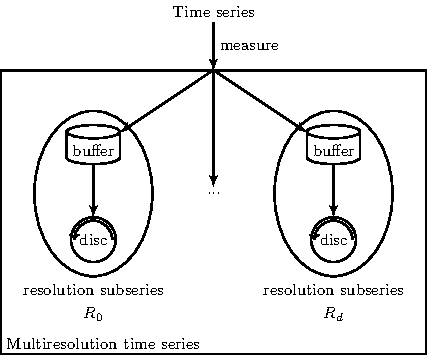
\includegraphics{fig_model_mtsdb.pdf}
  \caption{Architecture of \acro{MTSMS} model}
  \label{fig:model:mtsdb}
\end{figure}


In this way, the original time series gets stored spread in the discs,
each with a different time resolution and attribute aggregation.
Discs are size bounded so they only contain a fixed amount of
measures. When a disc becomes full it discards a measure. Thus,
multiresolution database is bounded in size and the time series gets
stored in pieces, that is time subseries.

Regarding operations, \acro{MTSMS} structure needs operators to change
the time intervals between measures and to select attributes. Mainly,
these operators are measure additions and time series consolidations,
which some functionality is delegated to operators called attribute
aggregate functions. Secondarily, there are operators to query the
multiresolution schema and extract time series data.


Following we define the \acro{MTSMS} model structure and structural
operators, the operations to query a multiresolution schema, and
attribute aggregate functions.  Furthermore, schema manipulation
operations could be defined but we focus on structure and data query .


\subsection{Structure}

A \emph{buffer} is a container for a regular or a irregular time
series. The buffer objective is to regularise the time series using a
predetermined step and an attribute function. We name
\emph{consolidation} to this action.
\begin{definition}%(Buffer)
  A \emph{buffer} is defined as the tuple $(S_B,\tau,\delta,f)$ where
  $S_B$ is a time series, $\tau$ is the last consolidation time,
  $\delta$ is the duration of the consolidation step and $f$ is an
  attribute aggregate function.

  An empty buffer $B_{\emptyset} = (\emptyset,t_0, \delta, f)$ has an
  empty time series, an initial consolidation time $t_0$ and
  predetermined $\delta$ and $f$.
\end{definition}

Operator \emph{addBuffer} adds a measure to its time series. Let $B=
(S_B,\tau,\delta,f)$ be a buffer and $m$ be a measure. $\addB: B
\times m \mapsto (S'_B,\tau,\delta,f)$ where $S'_B = S_B \cup \{m\} $.

From the $B_{\emptyset}$ all the consolidation time instants can be
calculated as $t_0+n\delta, n\in\N$. The consolidation of $B$ in a
time interval $I=[\tau,\tau+\delta]$ results in a measure
$m'=f(S_B,I)$ where $f$ is an attribute aggregate function
$f$. Operator \emph{consolidateBuffer} consolidates a set of measures
and removes the consolidated part of the time series from the
buffer. Let $B=(S_B,\tau,\delta,f)$ be a buffer. $\consB : B \mapsto
B' \times m'$ where $ B'= (S'_B,\tau+\delta,\delta,f)$, $m' =
f(S,[\tau,\tau+\delta])$, and $S'_B$ is the discarding of historic
data not needed anymore, for example $S'_B = S[\tau+\delta,+\infty]$.

On a simplified way, the \emph{consolidateBuffer} is only applied to the present
consolidation interval and the total consolidation is obtained by
successive application of the operator. This requires measures to be
added by time order and to consolidate the buffer when the time of
some measure is bigger than the buffer's next consolidation time.  Let
$B=(S_B,\tau,\delta,f)$ be a buffer and $m=\sup(S_B)$ the maximum
measure. $B$ is consolidable if and only if $T(m) \geq
\tau+\delta$.


A \emph{disc} is a finite capacity measures container. A time series
stored in a disc has its cardinal bounded. When the cardinal of the
time series is to overcome the limit, some measures need to be
discarded.
\begin{definition}%(Disc)
  A \emph{disc} is a tuple $(S_D,k)$ where $S_D$ is a time series and
  $k\in\N$ is the maximum allowed cardinal of $S_D$.  An empty disc
  $D_{\emptyset} = (\emptyset,k)$ has an empty time series and $k$ is
  the maximum cardinal allowed.
\end{definition}

The cardinal of the times series is kept under control by the add
operator. Let $D=(S_D,k)$ be a disc and $m$ be a measure. $\addD : D\times m\mapsto (S'_D,k)$ where %
$
 S_D' = \begin{cases}
  S_D\cup\{m\}                 & \text{if } |S_D|<k  \\
  (S_D-\{\min(S_D)\}) \cup \{m\} & \text{otherwise}
\end{cases}  
$.


A \emph{resolution subseries} is a structure that regularises and
aggregates a time series. It is composed of a buffer, that contains
the partial time series to be regularised, and a disc, that contains
the regularised time series.
\begin{definition}%(Resolution subseries)
  A \emph{resolution subseries} is a tuple $(B,D)$ where $B$ is a
  buffer and $D$ is a disc.  An empty buffer and empty disc imply an
  empty resolution subseries $R_{\emptyset} =
  (B_{\emptyset},D_{\emptyset})$.
\end{definition}
 
The operators of a resolution subseries extend the buffer and disc
ones. Let $R=(B,D)$ be a resolution subseries and $m$ be a measure.
(i) The addition of the measure to the buffer of the resolution
subseries: $\addR : R \times m \mapsto R'$ where $R'= (B',D)$,
and $B'= \addB(B,m)$. (ii) The consolidation of the resolution
subseries by consolidating its buffer and adding the consolidated
measure to its disc: $\consR : R \mapsto R'$ where $R'=
(B',D')$, $(B',m') = \consB(B)$, and $D'= \addD(D,m')$.  A resolution
subseries is consolidable only when its buffer is consolidable.




A \emph{multiresolution time series} is a set of resolution subseries
which share the input of measures, that is the same time series. A
time series is stored regularised and distributed with different
resolutions in the various resolution subseries, as previously shown
in Figure~\ref{fig:model:mtsdb}.
\begin{definition}%(Multiresolution time series)
  A \emph{Mul\-ti\-re\-solution time series} is a set of resolution
  subseries $\{R_0, \dots, R_d\}$.  An empty multiresolution series
  has empty resolution subseries $M_{\emptyset}=\{R_{0_\emptyset},
  \dots, R_{d_\emptyset}\}$. Usually there are no repeated pairs of
  ($\delta_i$,$f_i$) among a multiresolution series, so they act as a
  key attributes.
\end{definition}

Therefore, defining a multiresolution time series consists basically
in defining the quantity of resolution subseries and the
$(\delta,\tau,f,k)$ configuration parameters of each.


The operators of a multiresolution time series apply to every
resolution subseries contained. Let $M=\{R_0,\allowbreak
\dots,\allowbreak R_d\}$ be a multiresolution time series.  (i) The
addition of a measure to every resolution subseries: $\addM : M \times
m \mapsto \{R'_0, \dots,\allowbreak R'_d\}$ where
$R'_i=\addR(R_i,m)$. (ii) The consolidation of all resolution
subseries: $\consM : M \mapsto \{R'_0,\allowbreak \dots,\allowbreak
R'_d\}$ where $R'_i = \consR(R_i)$ if $R_i$ $\text{ consolidable}$ and
$R'_i=R_i$ $\text{otherwise}$.


The multiresolution consolidation operation should be applied
regularly based on a consolidation clock. When the measure ordered
addition approach is taken as explained in the buffer's consolidation,
then there is no need for a clock in a \acro{MTSMS}. The consolidation clock
is induced by the measure's addition and then it is only necessary to
check the multiresolution consolidation operation on new
additions. However, there could be other approaches where the
consolidation clock was given by an external clock or external
events. Then the consolidable definitions would depend on this
external clock.





\subsection{Queries}


There are two basic time series queries for a \acro{MTSMS}: (i) extract a
time subseries from a resolution subseries' disc or (ii) query for a
total time series from all consolidated data.

Let $M=\{R_0, \dots, R_d\}$ be a multiresolution time series and
$(\delta,f)$ be the key attributes. The first query selects a disc
from a multiresolution time series, $\seriedisc: M\times \delta \times
f \mapsto S'_D$ where $S'_D \in D' | (B',D') \in R',R' \in M$.

Let $M*=\{R_0, \dots, R_d\}$ be a multiresolution time series where
$R_i$ have a total order by their attribute $\delta_i$.  The second
query concatenates all discs' time subseries, $\totalseries: M*
\mapsto S'$ where $S' = S_{D0} || S_{D1} || \cdots || S_{Dd}$ and
$\delta_0 < \delta_1 < \cdots < \delta_d$. This query tries to obtain
the most resolution as possible, which is to say by $\delta$ order.
Being $(\delta,f)$ the key attributes, the $M*$ can be obtained from
$M$ by selecting resolution subseries with same $f$. If we operated a
$\totalseries$ to a general $M$ then it could be ambiguous as it could
contain repeated $\delta_i$.


From these two basic time series queries, more elaborated queries can
be applied to \acro{MTSMS} by using \acro{TSMS} operations. For
example, let $M_1$ and $M_2$ be two multiresolution time series, we
can compute the sum of both with $\totalseries(M_1) +
\totalseries(M_2)$.
% This is the general algebraic expressions that describes the model,
% but an implementation of the model could accomplish this operation
% in a more efficient way.





\subsection{Attribute aggregate function}
\label{sec:model:interpolador}

Attribute aggregate functions are a specific case of \acro{TSMS}
aggregate operations for summarising time series data when
consolidating a buffer. Let $S$ be a time series and $t_i$ and $t_j$
two time instants. An attribute aggregate function $f$ calculates a
measure that summarises the measures of $S$ included in the time
interval $I=[t_i,t_j]$:
\[
f : S=\{m_0,\ldots,m_k\} \times I=[t_i,t_j] \mapsto m'
\]
where, generally, $m'$ results from two operations on the time series:
(i) a time subseries selection $S'$ depending on the consolidating
interval, for example $S' = S[t_i,t_j]$, and (ii) a \acro{TSMS}
aggregation over this time subseries such as $m' = \agg(S',m, \fagg)$
where $\fagg$ is a function over two measures and $m$ an initial
measure.


Many different attribute aggregate functions can be used in order to
summarise a time series, for example it is possible to calculate an
statistic indicator of the time series such as the average or a more
complex digital signal processing operation
\cite{zhang11}. Furthermore, the representation for a time series and
some of its pathologies can be considered during the aggregation
process.


As it is possible to define many attribute aggregate
functions no global assumptions can be made about them. Each user has
to decide which combination of aggregation and representation fits
better with the measured phenomena.  Therefore, \acro{MTSMS} has to be
designed for allowing users to define aggregate functions.





Regarding the resulting consolidation time, normally it will be
$T(m')=t_j$ to be consistent with the consolidation operation of a
buffer where $\tau' = \tau + \delta \equiv t_j$. However $T(m')$ can
have a time offset with the buffer consolidating times, as instance
the resulting measure can be aggregated from a time subseries $S'$
with open interval $S'=S(t_i,t_j)$, closed interval $S'=S[t_i,t_j]$,
or other combinations like $S'=S(t_0-d,t_j-d]$ where $d$ is a time
duration.  The time offset can also be variable, as for example an
aggregate function that returns the first measure of the interval
$S[t_i,t_j)$, $m'=\min(S[t_i,t_j))$, then the resulting time can be
between $t_i \leq T(m') < t_j$.


Attribute general patterns can be defined that explain how the
resulting value $V(m')$ is calculated, letting the resulting time
instant $T(m')$ subject to interpretation.  Next there are some
attribute patterns examples based on temporal function time series
operators, that is the time series aggregated corresponds to a
continuous function $S(t)^r$ where $r$ is a representation as has been
described in Section~\ref{sec:model:tfunc}. The patterns of these
functions leave $T(m')$ undefined as well as the representation $r$ of
the time series. Let the time be continuous on all the time domain
$t\in T$:
\begin{itemize}
\item maximum$^r$: $S \times I \mapsto m'$ where $V(m') =
  \max\limits_{\forall t \in I}(S(t)^r)$. It summarises $S$ with the maximum
  of the measure values in the interval $I$.
\item last$^r$: $S \times I \mapsto m'$ where $V(m') = S(t_j)^r$. It
  summarises $S$ with the value at $t_j$ time instant.
\item mean$^r$: $S \times I \mapsto m'$ where $V(m') =
  \frac{1}{t_j-t_i} \int\limits_{t_i}^{t_j} S(t)^r dt$. It summarises $S$
  with the mean of the function in the interval $I$.
\end{itemize}


These aggregation function patterns can be expressed with discrete
mathematics for each particular representation, that is based on the
temporal interval defined in Section~\ref{sec:model:tfunc}. Next we
exemplify it by interpreting the general continuous patterns for two
particular representations that have been defined previously: \dd{}
and \zohe{}.


Dirac delta attribute aggregation functions $f^\dd$ have a general
form $f^\dd : S \times [t_i,t_j]\mapsto m'$ where $m'=(t',v')$, the
resulting time is interpreted as centred on the interval
$t'=\frac{t_j+t_i}{2}$ and the resulting value depends on the
attribute, let $S'=S[t_i,t_j]^\dd$ be the selection of measures by
Dirac delta temporal interval:
\begin{itemize}
\item maximum$^\dd$: $v' = \max\big(0,\max_{\forall m \in S'}(V(m))\big)$. 
\item last$^\dd$: $v' = V(\max(S'))$.
\item mean$^\dd$: $v' = \frac{1}{t_j-t_i} \sum\limits_{\forall m
    \in S'} V(m)$, as Dirac delta function has property $\int\dd(t)dt=1$.
\end{itemize}

With reference to \acro{TSMS} aggregation, $\max(S')$ is an operator
defined in Section~\ref{sec:model:operations}. The remaining
operations could be implemented with aggregation operations. As
instance, $\sum\limits_{\forall m \in S'} V(m)$ is a sum of values
that could be implemented as $\agg(S',(0,0),\fagg)$ where $\fagg:
(t_a,v_a) \times (t_b,v_b) \mapsto (0,v_a+v_b)$ as showed in
Example~\ref{ex:computational-operators}.



\zohe{} attribute aggregation functions $f^\zohe{}$ have a general
form $f^\zohe{} : S \times [t_i,t_j]\mapsto m'$ where $m'=(t',v')$,
the resulting time is interpreted as right limit of the interval
$t'=t_j$ and the resulting value depends on the attribute, let
$S'=S[t_i,t_j]^\zohe{}$ be the selection of measures by \zohe{} temporal
interval:
\begin{itemize}
\item maximum$^\zohe{}$: $v' = \max_{\forall m \in S'}(V(m))$. 
\item last$^\zohe{}$: $v' = V(\max(S'))$.
\item mean$^\zohe{}$: $v' = \frac{1}{t_j-t_i} \big[ (T(o)-t_0)V(o) +
  \sum\limits_{\forall m \in S''}( T(m)- T(\prev_S
  m) )V(m) \big]$ where $o=\min(S')$ and $S''= S' - \{o\}$.
\end{itemize}

A similar aggregation function to mean$^\zohe{}$ is used by \emph{RRDtool}
\cite{rrdtool} in order to summarise velocity coun\-ter
data by keeping the total counting information, as mean aggregation
can be seen as one keeping the area below the original signal.


In conclusion, some patterns are very similar. As instance maximum and
last attributes differ basically on the interval selection
operation. However, other patterns have a more elaborated
interpretation in a particular representation. As instance
mean$^\zohe{}$ and mean$^\dd$ are an elaborated interpretation for
the general integral definition.





\begin{example}\label{ex:model:smultiresolution} 
  We define a multiresolution schema for a time series, we consolidate
  the database and we query its data.  Let $S = \{
  (1,6),(5,2),\allowbreak (8,5),\allowbreak (10,0),\allowbreak
  (14,1),\allowbreak (19,6),\allowbreak (22,11),\allowbreak
  (26,6),(29,0) \}$ be a time series and $M_\emptyset=\{R_0,R_1\}$ a
  multiresolution time series where each resolution parameters are
  $\tau_0=0$ , $\delta_0=5$, $f_0 =\meanz$, $k_0=4$ and $\tau_1=0$,
  $\delta_1=10$, $f_1 =\maxz$, $k_1=2$. Therefore $R_0$ will be
  consolidated at time instants 5, 10, 15, 20, 25, 30\dots and $R_1$
  at 10, 20, 30\dots

  All measures of $S$ are added to $M_\emptyset$
  and then it is consolidated until it is no more consolidable. As
  $T(\max(S))=29$, the last consolidation times are $\tau_0=25$ and
  $\tau_1=20$, so we call $M_{29}$ to this multiresolution time series
  at this state.

  Then the two time subseries consolidated are obtained by querying
  $\seriedisc(M_{29},5,\allowbreak \meanz)=\{(10,3),\allowbreak
  (15,\allowbreak 2),\allowbreak (20,7),\allowbreak (25,8)\}$ and
  $\seriedisc(M_{29},10,\allowbreak  \maxz) =\allowbreak \{ \allowbreak
  (10,6),\allowbreak (20,11)\}$. Regarding buffers, note that
  $S_{B0_{29}}= \{\allowbreak (26,6),\allowbreak (29,0)\allowbreak \}$
  and $S_{B1_{29}}=\{\allowbreak (22,11),\allowbreak (26,6),(29,0)\}$.

  In this particular example
  $ \totalseries(M_{29}) = \seriedisc(M_{29},\allowbreak 5,\meanz)$ as $R_0$ has
  double resolution than $R_1$. 
\end{example}



%%% Local Variables:
%%% TeX-master: "main"
%%% ispell-local-dictionary: "british"
%%% End:

% LocalWords:  genericity multiresolution subseries consolidable MTSM

% LocalWords:  pathologies MTSMS TSMS cardinality multivalued infimum
% LocalWords:  multivalues supremum
